\documentclass[ignorenonframetext,]{beamer}
\setbeamertemplate{caption}[numbered]
\setbeamertemplate{caption label separator}{: }
\setbeamercolor{caption name}{fg=normal text.fg}
\beamertemplatenavigationsymbolsempty
\usepackage{lmodern}
\usepackage{amssymb,amsmath}
\usepackage{ifxetex,ifluatex}
\usepackage{fixltx2e} % provides \textsubscript
\ifnum 0\ifxetex 1\fi\ifluatex 1\fi=0 % if pdftex
  \usepackage[T1]{fontenc}
  \usepackage[utf8]{inputenc}
\else % if luatex or xelatex
  \ifxetex
    \usepackage{mathspec}
  \else
    \usepackage{fontspec}
  \fi
  \defaultfontfeatures{Ligatures=TeX,Scale=MatchLowercase}
\fi
% use upquote if available, for straight quotes in verbatim environments
\IfFileExists{upquote.sty}{\usepackage{upquote}}{}
% use microtype if available
\IfFileExists{microtype.sty}{%
\usepackage{microtype}
\UseMicrotypeSet[protrusion]{basicmath} % disable protrusion for tt fonts
}{}
\newif\ifbibliography
\hypersetup{
            pdfborder={0 0 0},
            breaklinks=true}
\usepackage{longtable,booktabs}
\usepackage{caption}
% These lines are needed to make table captions work with longtable:
\makeatletter
\def\fnum@table{\tablename~\thetable}
\makeatother

% Prevent slide breaks in the middle of a paragraph:
\widowpenalties 1 10000
\raggedbottom

\AtBeginPart{
  \let\insertpartnumber\relax
  \let\partname\relax
  \frame{\partpage}
}
\AtBeginSection{
  \ifbibliography
  \else
    \let\insertsectionnumber\relax
    \let\sectionname\relax
    \frame{\sectionpage}
  \fi
}
\AtBeginSubsection{
  \let\insertsubsectionnumber\relax
  \let\subsectionname\relax
  \frame{\subsectionpage}
}

\setlength{\parindent}{0pt}
\setlength{\parskip}{6pt plus 2pt minus 1pt}
\setlength{\emergencystretch}{3em}  % prevent overfull lines
\providecommand{\tightlist}{%
  \setlength{\itemsep}{0pt}\setlength{\parskip}{0pt}}
\setcounter{secnumdepth}{0}
\usepackage[british]{babel}
\usepackage{graphicx,hyperref,anderson,url}
\usepackage{fontawesome}

\title[Assessing hurricane exposure for epidemiology]{Assessing exposure to hurricanes and other tropical
storms for epidemiological research}
\subtitle{Drexel University Environmental and Occupational Health Research Seminar}
\date{January 11, 2017}

\author[Brooke Anderson]{
  Brooke Anderson \\\medskip
  {\small \faEnvelope: \url{brooke.anderson@colostate.edu}} \\
  {\small \faGithub:  \url{www.github.com/geanders}}}

\institute[Colorado State University]{
  Department of Environmental \& Radiological Health Sciences \\
  Environmental Epidemiology Section \\
  Colorado State University}

\date{}

\begin{document}

\begin{frame}
  \titlepage
\end{frame}

\section{Motivation}\label{motivation}

\section{Assessing exposure}\label{assessing-exposure}

\begin{frame}{Study data}

\begin{center}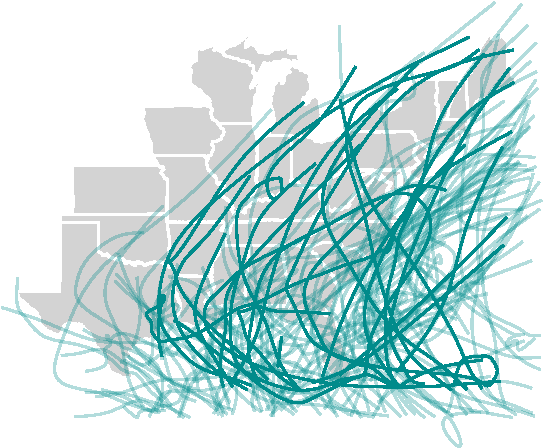
\includegraphics[width=0.75\textwidth]{anderson_jan11_files/figure-beamer/unnamed-chunk-1-1} \end{center}

\end{frame}

\begin{frame}{Hazard-specific metrics}

\begin{columns}
\begin{column}{0.5\textwidth}
\begin{block}{Tropical storm hazard metrics}
   \begin{itemize}
    \item Distance from the storm
    \item High winds
    \item Rainfall
    \item Flood events
    \item Tornado events
   \end{itemize}
\end{block}
\end{column}
\begin{column}{0.5\textwidth}  
    \vspace{-0.25cm}
    \begin{center}
     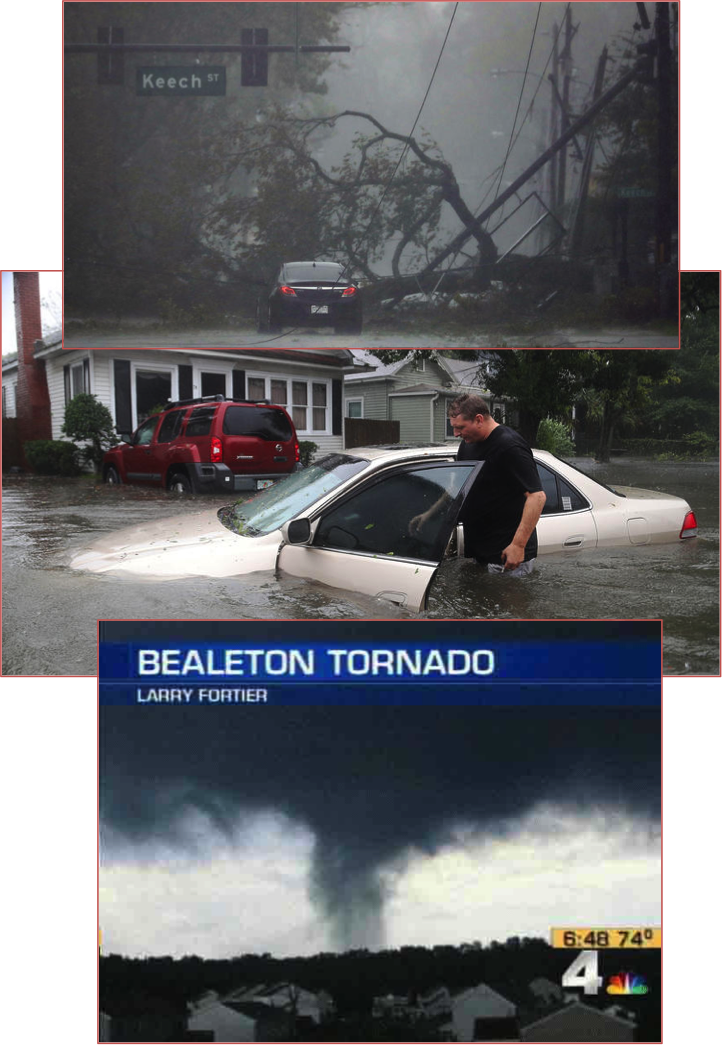
\includegraphics[width=0.8\textwidth]{storm_hazards.png}
     \end{center}
     \vspace{-0.25cm}
     \scriptsize{Image sources: Los Angeles Times, NBC}
\end{column}
\end{columns}

\end{frame}

\begin{frame}{Distance from storm}

{[}Intro to best tracks{]}

\end{frame}

\begin{frame}{Distance from storm}

{[}Importance of interpolating tracks{]}

\end{frame}

\begin{frame}{Wind exposure}

{[}Reminder of best tracks, intro to Willoughby model{]}

\end{frame}

\begin{frame}{Wind exposure}

{[}Factors of doing the modeling (transfering from surface to gradient
and back, etc.), other applications of the model{]}

\end{frame}

\begin{frame}{Wind exposure}

Wind radii from Extended Best Tracks data for Katrina

\begin{flushleft}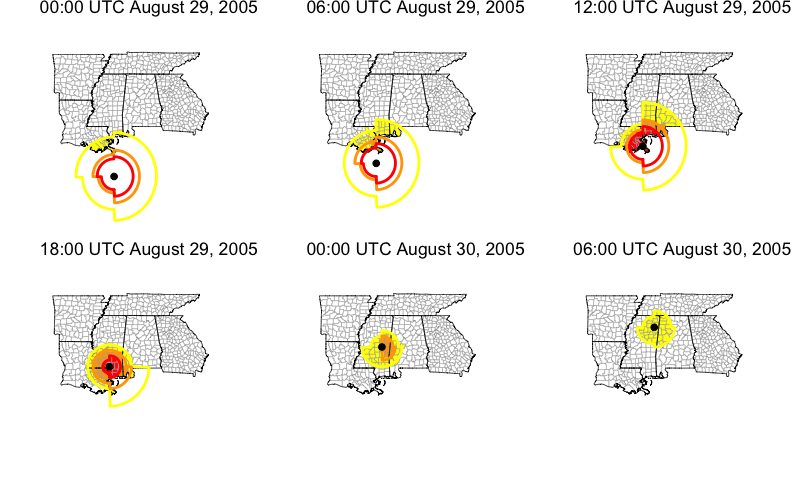
\includegraphics[width=1.03\textwidth]{ext_tracks_3} \end{flushleft}

\end{frame}

\begin{frame}{Wind exposure}

Evaluating wind model: Hurricane Katrina, 2005

\begin{flushleft}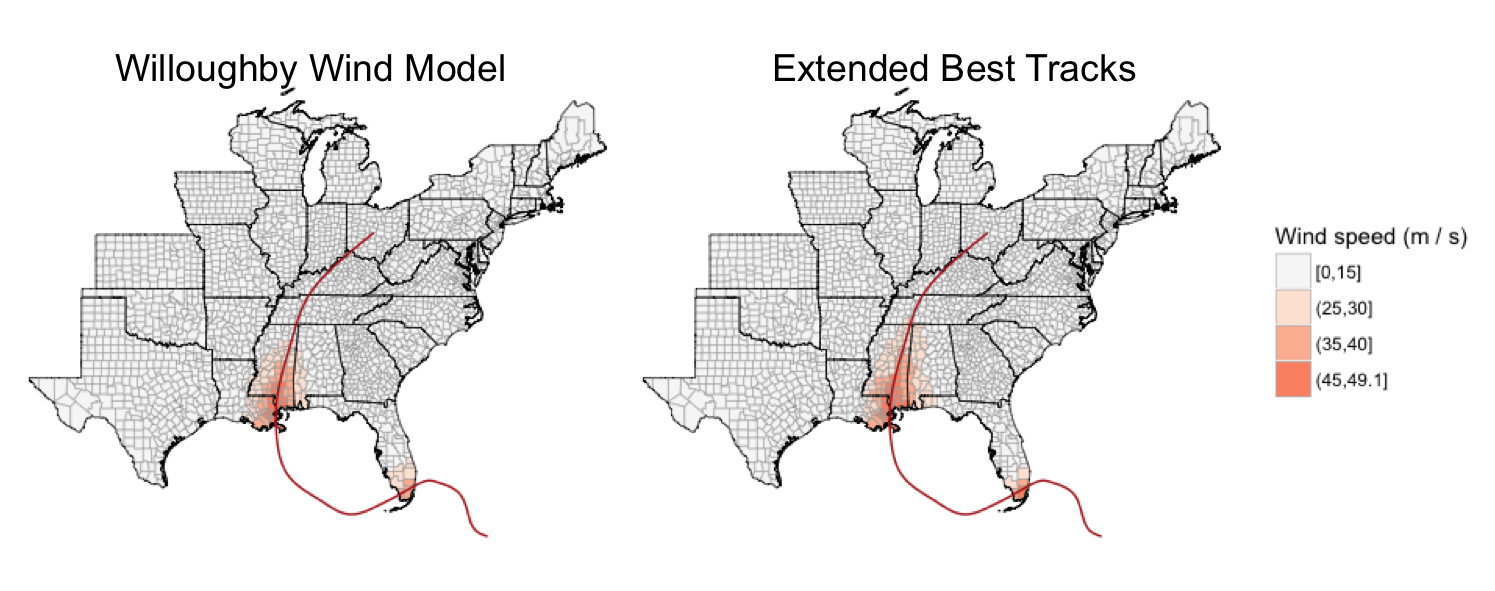
\includegraphics[width=1.05\textwidth]{wind_model_eval_katrina_2005} \end{flushleft}

\end{frame}

\begin{frame}{Wind exposure}

Evaluating wind model: Hurricane Ike, 2008

\begin{flushleft}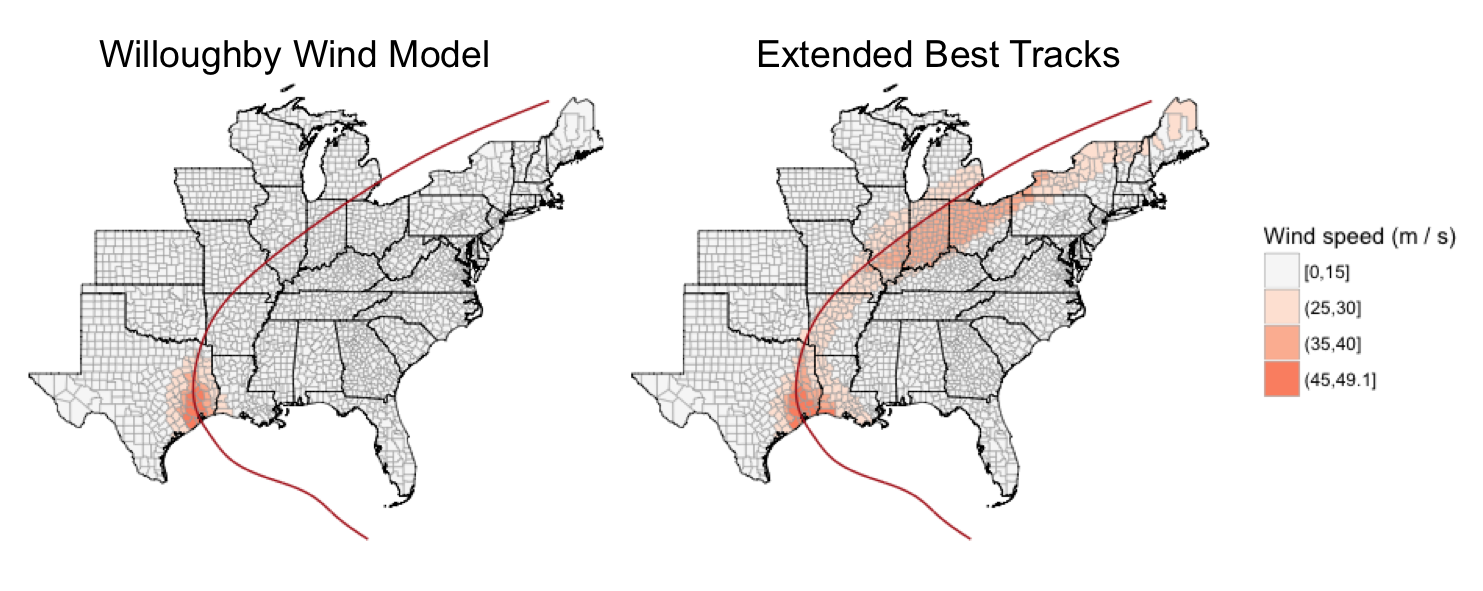
\includegraphics[width=1.05\textwidth]{wind_model_eval_ike_2008} \end{flushleft}

\end{frame}

\begin{frame}{Wind exposure}

Evaluating wind model: Hurricane Sandy, 2012

\begin{flushleft}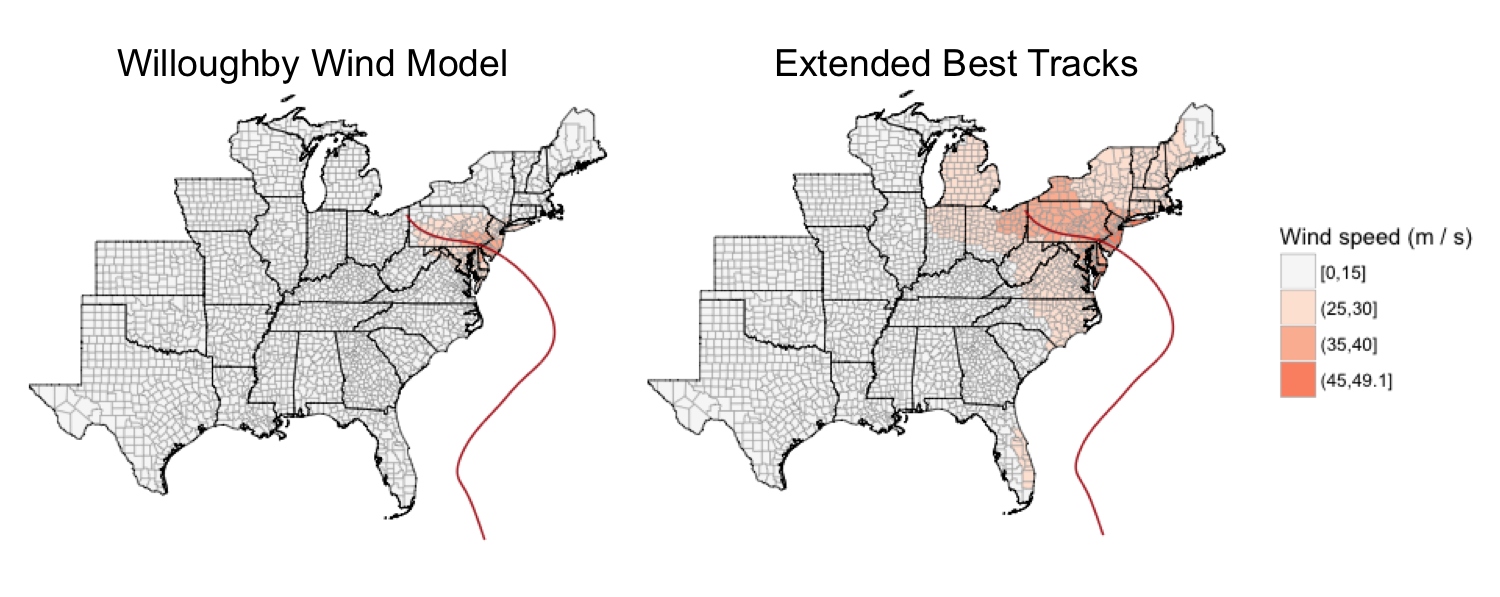
\includegraphics[width=1.05\textwidth]{wind_model_eval_sandy_2012} \end{flushleft}

\end{frame}

\begin{frame}{Rain exposure}

\begin{columns}
\begin{column}{0.35\textwidth}
\footnotesize
\begin{block}{NLDAS-2 precipitation}
  \begin{itemize}
  \item Find out more: http://ldas.gsfc.nasa.gov/nldas/
  \item Also available at county-level through CDC Wonder: https://wonder.cdc.gov
  \end{itemize}
\end{block}
\end{column}
\begin{column}{0.65\textwidth}  
    \vspace{-0.25cm}
    NLDAS-2 precipitation data for Tropical Storm Lee
    \begin{center}
     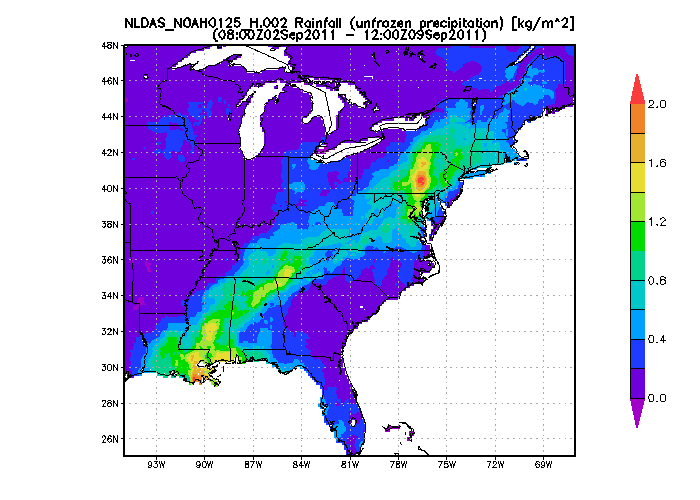
\includegraphics[width=\textwidth]{nldas2_ts_lee.png}
     \end{center}
     \vspace{-0.25cm}
     \scriptsize{Image source: Goddard Earth Sciences DISC}
\end{column}
\end{columns}

\end{frame}

\begin{frame}{Rain exposure}

{[}Showing how to ID date of closest approach{]}

\end{frame}

\begin{frame}{Rain exposure}

\begin{flushleft}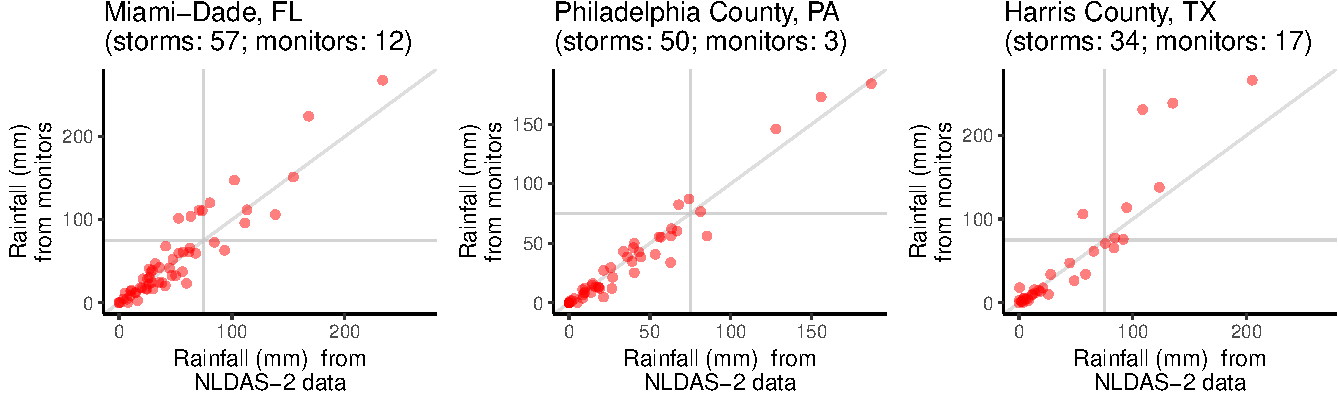
\includegraphics[width=1.05\textwidth]{anderson_jan11_files/figure-beamer/compare_rain_ex_counties-1} \end{flushleft}

\end{frame}

\begin{frame}{Rain exposure}

\begin{center}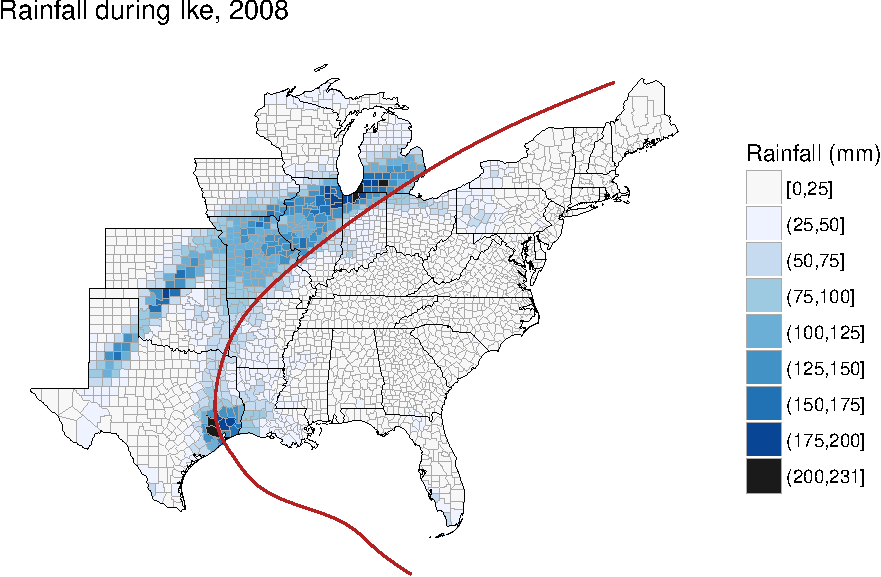
\includegraphics[width=0.9\textwidth]{anderson_jan11_files/figure-beamer/ike_rain_example-1} \end{center}

\end{frame}

\begin{frame}{Rain exposure}

\begin{center}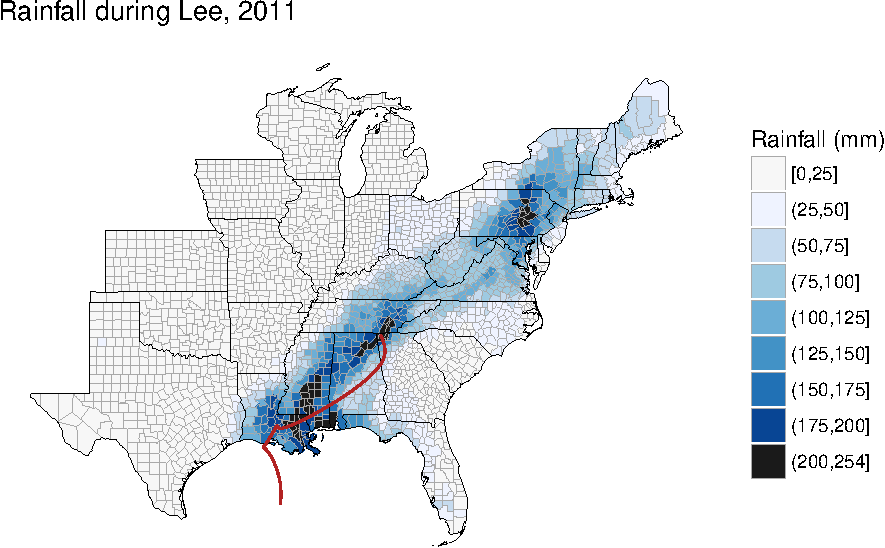
\includegraphics[width=0.9\textwidth]{anderson_jan11_files/figure-beamer/lee_rain_example-1} \end{center}

\end{frame}

\begin{frame}{Flood and tornado events}

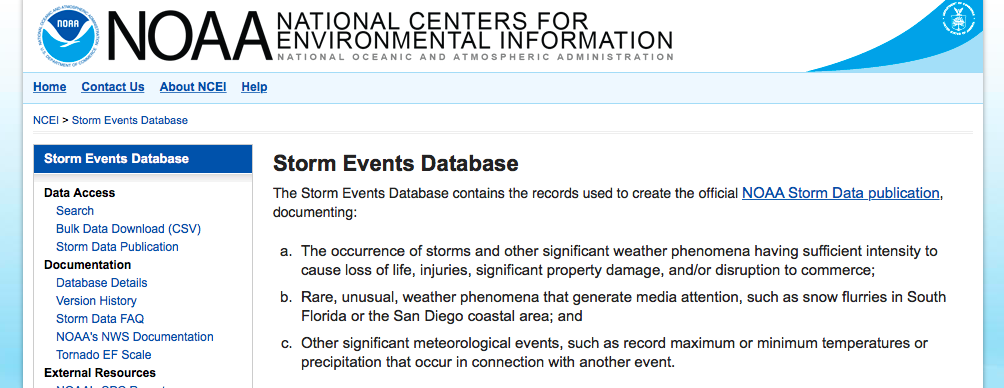
\includegraphics[width=\textwidth]{noaastormevents}

Website: \url{https://www.ncdc.noaa.gov/stormevents/}

\end{frame}

\begin{frame}{Flood and tornado events}

\begin{center}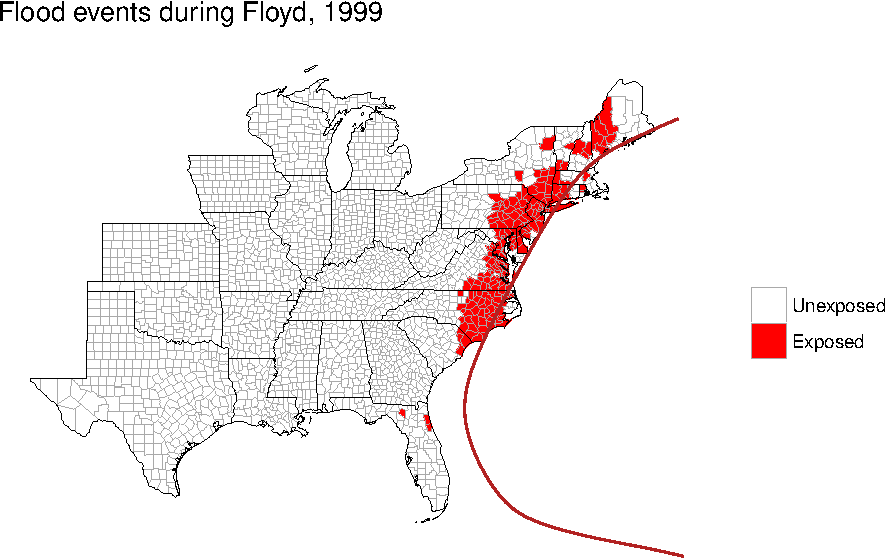
\includegraphics[width=0.9\textwidth]{anderson_jan11_files/figure-beamer/floyd_flood_example-1} \end{center}

\end{frame}

\begin{frame}{Flood and tornado events}

\begin{center}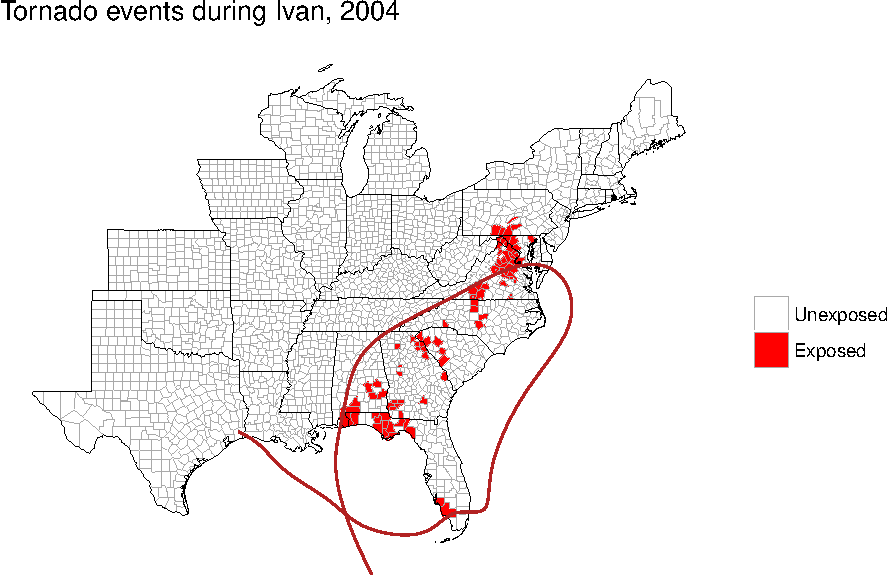
\includegraphics[width=0.9\textwidth]{anderson_jan11_files/figure-beamer/ivan_tornado_example-1} \end{center}

\end{frame}

\section{Agreement between exposure
metrics}\label{agreement-between-exposure-metrics}

\begin{frame}{Storm exposure}

\footnotesize

\begin{longtable}[]{@{}ll@{}}
\toprule
\begin{minipage}[b]{0.24\columnwidth}\raggedright\strut
Exposure metric\strut
\end{minipage} & \begin{minipage}[b]{0.65\columnwidth}\raggedright\strut
Criterial for exposure\strut
\end{minipage}\tabularnewline
\midrule
\endhead
\begin{minipage}[t]{0.24\columnwidth}\raggedright\strut
Distance\strut
\end{minipage} & \begin{minipage}[t]{0.65\columnwidth}\raggedright\strut
County population mean center within 100 km of storm track\strut
\end{minipage}\tabularnewline
\begin{minipage}[t]{0.24\columnwidth}\raggedright\strut
Rain\strut
\end{minipage} & \begin{minipage}[t]{0.65\columnwidth}\raggedright\strut
County received 75 mm or more rain over the period from two days before
to one day after the storm's closest approach and the storm passed
within 500 km of the county\strut
\end{minipage}\tabularnewline
\begin{minipage}[t]{0.24\columnwidth}\raggedright\strut
Wind\strut
\end{minipage} & \begin{minipage}[t]{0.65\columnwidth}\raggedright\strut
Modeled wind speed at county's population mean center met or exceeded 15
m / s during the storm\strut
\end{minipage}\tabularnewline
\begin{minipage}[t]{0.24\columnwidth}\raggedright\strut
Flood\strut
\end{minipage} & \begin{minipage}[t]{0.65\columnwidth}\raggedright\strut
Flood event listed with a start date within two days of the storm's
closest approach and county within 500 km of storm track\strut
\end{minipage}\tabularnewline
\begin{minipage}[t]{0.24\columnwidth}\raggedright\strut
Tornado\strut
\end{minipage} & \begin{minipage}[t]{0.65\columnwidth}\raggedright\strut
Tornado event listed with a start date within two days of the storm's
closest approach and county within 500 km of storm track\strut
\end{minipage}\tabularnewline
\bottomrule
\end{longtable}

\end{frame}

\begin{frame}{Storm exposure}

\begin{longtable}[]{@{}lcc@{}}
\toprule
\begin{minipage}[b]{0.23\columnwidth}\raggedright\strut
Exposure metric\strut
\end{minipage} & \begin{minipage}[b]{0.34\columnwidth}\centering\strut
Median number of exposed counties (IQR)\strut
\end{minipage} & \begin{minipage}[b]{0.34\columnwidth}\centering\strut
Storm with most counties exposed\strut
\end{minipage}\tabularnewline
\midrule
\endhead
\begin{minipage}[t]{0.23\columnwidth}\raggedright\strut
Distance\strut
\end{minipage} & \begin{minipage}[t]{0.34\columnwidth}\centering\strut
62 (12, 156)\strut
\end{minipage} & \begin{minipage}[t]{0.34\columnwidth}\centering\strut
Beryl, 1994 (330)\strut
\end{minipage}\tabularnewline
\begin{minipage}[t]{0.23\columnwidth}\raggedright\strut
Rain\strut
\end{minipage} & \begin{minipage}[t]{0.34\columnwidth}\centering\strut
32 (4, 133)\strut
\end{minipage} & \begin{minipage}[t]{0.34\columnwidth}\centering\strut
Frances, 2004 (464)\strut
\end{minipage}\tabularnewline
\begin{minipage}[t]{0.23\columnwidth}\raggedright\strut
Wind\strut
\end{minipage} & \begin{minipage}[t]{0.34\columnwidth}\centering\strut
26 (3, 65)\strut
\end{minipage} & \begin{minipage}[t]{0.34\columnwidth}\centering\strut
Ike, 2008 (355)\strut
\end{minipage}\tabularnewline
\begin{minipage}[t]{0.23\columnwidth}\raggedright\strut
Flood\strut
\end{minipage} & \begin{minipage}[t]{0.34\columnwidth}\centering\strut
9 (0, 39)\strut
\end{minipage} & \begin{minipage}[t]{0.34\columnwidth}\centering\strut
Ivan, 2004 (317)\strut
\end{minipage}\tabularnewline
\begin{minipage}[t]{0.23\columnwidth}\raggedright\strut
Tornado\strut
\end{minipage} & \begin{minipage}[t]{0.34\columnwidth}\centering\strut
1 (0, 9)\strut
\end{minipage} & \begin{minipage}[t]{0.34\columnwidth}\centering\strut
Ivan, 2004 (91)\strut
\end{minipage}\tabularnewline
\bottomrule
\end{longtable}

\footnotesize{\textsuperscript{*}Note: Flood and Tornado events only include storms in 1996--2011. All other event listings cover storms in 1988--2011.}

\end{frame}

\begin{frame}{Storm-specific severity}

{[}How we measured this: Spearman's rank correlation{]}

\end{frame}

\begin{frame}{Storm-specific severity}

\begin{center}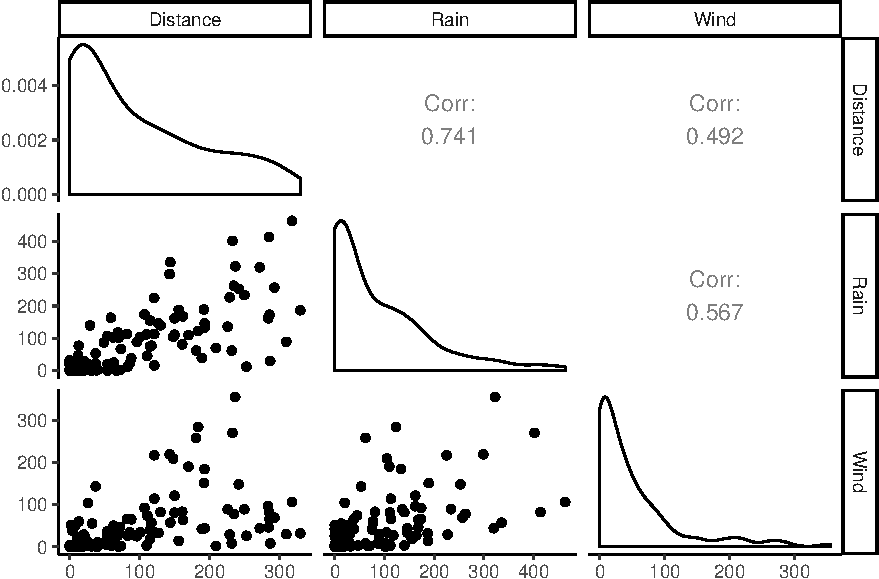
\includegraphics[width=0.8\textwidth]{anderson_jan11_files/figure-beamer/unnamed-chunk-10-1} \end{center}

\end{frame}

\begin{frame}{Storm-specific severity}

\begin{longtable}[]{@{}cccccc@{}}
\toprule
\begin{minipage}[b]{0.17\columnwidth}\centering\strut
~\strut
\end{minipage} & \begin{minipage}[b]{0.13\columnwidth}\centering\strut
Distance\strut
\end{minipage} & \begin{minipage}[b]{0.08\columnwidth}\centering\strut
Rain\strut
\end{minipage} & \begin{minipage}[b]{0.08\columnwidth}\centering\strut
Wind\strut
\end{minipage} & \begin{minipage}[b]{0.09\columnwidth}\centering\strut
Flood\strut
\end{minipage} & \begin{minipage}[b]{0.10\columnwidth}\centering\strut
Tornado\strut
\end{minipage}\tabularnewline
\midrule
\endhead
\begin{minipage}[t]{0.17\columnwidth}\centering\strut
\textbf{Distance}\strut
\end{minipage} & \begin{minipage}[t]{0.13\columnwidth}\centering\strut
-\strut
\end{minipage} & \begin{minipage}[t]{0.08\columnwidth}\centering\strut
-\strut
\end{minipage} & \begin{minipage}[t]{0.08\columnwidth}\centering\strut
-\strut
\end{minipage} & \begin{minipage}[t]{0.09\columnwidth}\centering\strut
-\strut
\end{minipage} & \begin{minipage}[t]{0.10\columnwidth}\centering\strut
-\strut
\end{minipage}\tabularnewline
\begin{minipage}[t]{0.17\columnwidth}\centering\strut
\textbf{Rain}\strut
\end{minipage} & \begin{minipage}[t]{0.13\columnwidth}\centering\strut
0.79\strut
\end{minipage} & \begin{minipage}[t]{0.08\columnwidth}\centering\strut
-\strut
\end{minipage} & \begin{minipage}[t]{0.08\columnwidth}\centering\strut
-\strut
\end{minipage} & \begin{minipage}[t]{0.09\columnwidth}\centering\strut
-\strut
\end{minipage} & \begin{minipage}[t]{0.10\columnwidth}\centering\strut
-\strut
\end{minipage}\tabularnewline
\begin{minipage}[t]{0.17\columnwidth}\centering\strut
\textbf{Wind}\strut
\end{minipage} & \begin{minipage}[t]{0.13\columnwidth}\centering\strut
0.71\strut
\end{minipage} & \begin{minipage}[t]{0.08\columnwidth}\centering\strut
0.69\strut
\end{minipage} & \begin{minipage}[t]{0.08\columnwidth}\centering\strut
-\strut
\end{minipage} & \begin{minipage}[t]{0.09\columnwidth}\centering\strut
-\strut
\end{minipage} & \begin{minipage}[t]{0.10\columnwidth}\centering\strut
-\strut
\end{minipage}\tabularnewline
\begin{minipage}[t]{0.17\columnwidth}\centering\strut
\textbf{Flood}\strut
\end{minipage} & \begin{minipage}[t]{0.13\columnwidth}\centering\strut
0.46\strut
\end{minipage} & \begin{minipage}[t]{0.08\columnwidth}\centering\strut
0.54\strut
\end{minipage} & \begin{minipage}[t]{0.08\columnwidth}\centering\strut
0.44\strut
\end{minipage} & \begin{minipage}[t]{0.09\columnwidth}\centering\strut
-\strut
\end{minipage} & \begin{minipage}[t]{0.10\columnwidth}\centering\strut
-\strut
\end{minipage}\tabularnewline
\begin{minipage}[t]{0.17\columnwidth}\centering\strut
\textbf{Tornado}\strut
\end{minipage} & \begin{minipage}[t]{0.13\columnwidth}\centering\strut
0.43\strut
\end{minipage} & \begin{minipage}[t]{0.08\columnwidth}\centering\strut
0.50\strut
\end{minipage} & \begin{minipage}[t]{0.08\columnwidth}\centering\strut
0.45\strut
\end{minipage} & \begin{minipage}[t]{0.09\columnwidth}\centering\strut
0.78\strut
\end{minipage} & \begin{minipage}[t]{0.10\columnwidth}\centering\strut
-\strut
\end{minipage}\tabularnewline
\bottomrule
\end{longtable}

\end{frame}

\begin{frame}{County-specific classification}

We measured agreement in county-specific exposure classifications for
different storm hazards using \textbf{Cohen's Kappa}:

\[
\kappa = \frac{p_{o} - p_{e}}{1 - p_{e}}
\]

where:

\begin{itemize}
\tightlist
\item
  \(p_o\): Observed agreement between two hazard classifications
\item
  \(p_e\): Expected agreement between two hazard classifications if
  ratings were independent
\end{itemize}

\end{frame}

\begin{frame}{County-specific classification}

{[}What we found{]}

\end{frame}

\begin{frame}{Discussion}

\end{frame}

\section{Software}\label{software}

\begin{frame}{Software as a research product}

{[}Open science, ROpenSci, influence of example packages{]}

\end{frame}

\begin{frame}{Software as a research product}


\includegraphics[width=\textwidth]{coursera_screenshot}
\url{https://www.coursera.org/specializations/r}
\url{https://bookdown.org/rdpeng/RProgDA/}

\end{frame}

\begin{frame}{Project software}

{[}list of software, availability through CRAN, GitHub{]}

\end{frame}

\begin{frame}[fragile]{Sharing exposure data}

{[}\texttt{hurricaneexposure}, \texttt{hurricaneexposuredata}, web
page{]}

\end{frame}

\begin{frame}[fragile]{Modeling storm winds}

{[}\texttt{stormwindmodel}{]}

\end{frame}

\begin{frame}[fragile]{Working with NOAA Storm Events}

{[}\texttt{noaastormevents}{]}

\end{frame}

\begin{frame}[fragile]{Dealing with time zones}

{[}\texttt{countytimezones}{]}

\end{frame}

\end{document}
